\subsection{ISO 9001:2015}
	\subsubsection{Generalidades}
		\par 
			La adopción de un sistema de gestión de la calidad es una decisión estratégica para una organización
			que le puede ayudar a mejorar su desempeño global y proporcionar una base sólida para las iniciativas
			de desarrollo sostenible.
		
		\par \noindent
			Los requisitos del sistema de gestión de la calidad especificados en esta Norma Internacional son
			complementarios a los requisitos para los productos y servicios.
			
		\par \noindent
			Esta Norma Internacional emplea el enfoque a procesos, que incorpora el ciclo Planificar-HacerVerificar-Actuar (PHVA) y el pensamiento basado en riesgos.
			
		\par \noindent
			El enfoque a procesos permite a una organización planificar sus procesos y sus interacciones.
			El ciclo PHVA permite a una organización asegurarse de que sus procesos cuenten con recursos y se
			gestionen adecuadamente, y que las oportunidades de mejora se determinen y se actúe en consecuencia.
			
		\par \noindent
			El pensamiento basado en riesgos permite a una organización determinar los factores que podrían
			causar que sus procesos y su sistema de gestión de la calidad se desvíen de los resultados planificados,
			para poner en marcha controles preventivos para minimizar los efectos negativos y maximizar el uso
			de las oportunidades a medida que surjan.
			
	\paragraph{Enfoque a procesos}
	
		Esta Norma Internacional promueve la adopción de un enfoque a procesos al desarrollar, implementar
		y mejorar la eficacia de un sistema de gestión de la calidad, para aumentar la satisfacción del cliente
		mediante el cumplimiento de los requisitos del cliente.
	
		\par \noindent	
			La comprensión y gestión de los procesos interrelacionados como un sistema contribuye a la eficacia
			y eficiencia de la organización en el logro de sus resultados previstos. Este enfoque permite a la
			organización controlar las interrelaciones e interdependencias entre los procesos del sistema, de modo
			que se pueda mejorar el desempeño global de la organización.
		
\newpage
\thispagestyle{plain}
		
		\par \noindent
			El enfoque a procesos implica la definición y gestión sistemática de los procesos y sus interacciones,
			con el fin de alcanzar los resultados previstos de acuerdo con la política de la calidad y la dirección
			estratégica de la organización. La gestión de los procesos y el sistema en su conjunto puede alcanzarse
			utilizando el ciclo PHVA con un enfoque global de pensamiento basado en riesgos dirigido a aprovechar las oportunidades y prevenir resultados no deseados.
		
		\par \noindent
			La aplicación del enfoque a procesos en un sistema de gestión de la calidad permite:
			
		\begin{itemize}
			
			\item la comprensión y la coherencia en el cumplimiento de los requisitos;
			
			\item la consideración de los procesos en términos de valor agregado;
			
			\item el logro del desempeño eficaz del proceso;
			
			\item la mejora de los procesos con base en la evaluación de los datos y la información.
			
		\end{itemize}

		\begin{figure}[h]
			\centering
			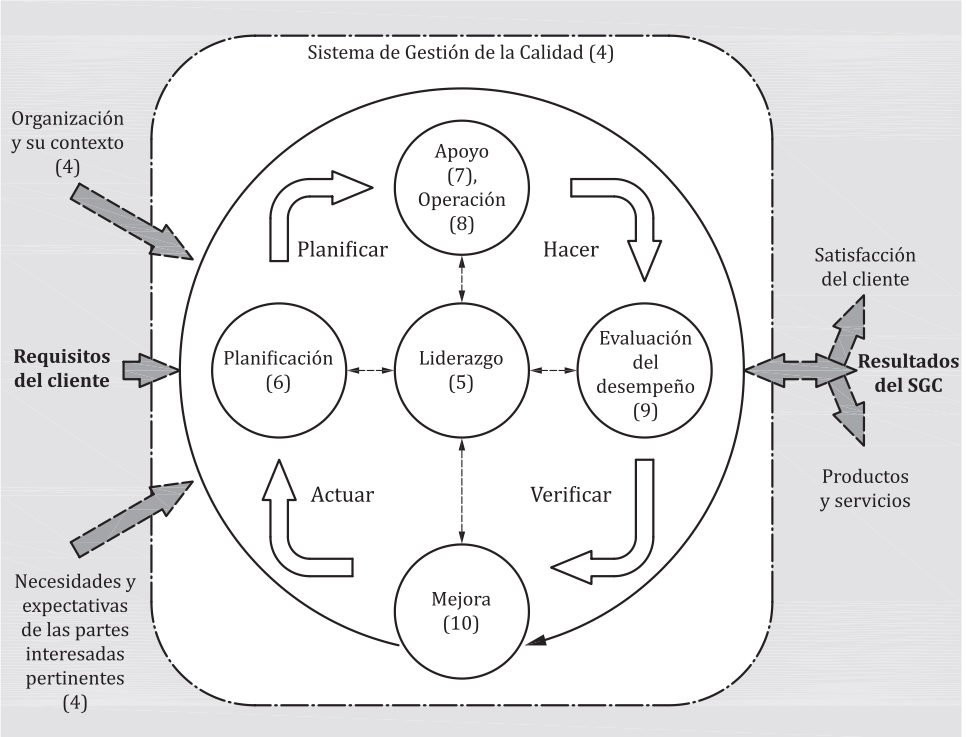
\includegraphics[width=12cm, height=10cm]{figura1.png}
			\caption{Ilustración del ciclo Planificar-Hacer-Verificar-Actuar}
		\end{figure}

\newpage
\thispagestyle{plain}

		\par \noindent
			El ciclo PHVA puede describirse brevemente como sigue:
		\begin{itemize}
			\item Planificar: establecer los objetivos del sistema y sus procesos, y los recursos necesarios para
			generar y proporcionar resultados de acuerdo con los requisitos del cliente y las políticas de la
			organización, e identificar y abordar los riesgos y las oportunidades;
			
			\item Hacer: implementar lo planificado;
			
			\item Verificar: realizar el seguimiento y (cuando sea aplicable) la medición de los procesos y los productos
			y servicios resultantes respecto a las políticas, los objetivos, los requisitos y las actividades
			planificadas, e informar sobre los resultados;
			
			\item Actuar: tomar acciones para mejorar el desempeño, cuando sea necesario.
		\end{itemize}
		
	\paragraph{Pensamiento basado en riesgos}
		
		El pensamiento basado en riesgos es esencial para lograr un sistema de gestión de la calidad eficaz. El concepto de pensamiento basado en riesgos ha estado implícito en ediciones anteriores de esta Norma Internacional, incluyendo, por ejemplo, llevar a cabo acciones preventivas para eliminar no conformidades potenciales, analizar cualquier no conformidad que ocurra, y tomar acciones que sean apropiadas para los efectos de la no conformidad para prevenir su recurrencia.
		
		\par \noindent
			Para ser conforme con los requisitos de esta Norma Internacional, una organización necesita planificar
			e implementar acciones para abordar los riesgos y las oportunidades. Abordar tanto los riesgos como
			las oportunidades establece una base para aumentar la eficacia del sistema de gestión de la calidad,
			alcanzar mejores resultados y prevenir los efectos negativos.
		
		\par \noindent
			Las oportunidades pueden surgir como resultado de una situación favorable para lograr un resultado
			previsto, por ejemplo, un conjunto de circunstancias que permita a la organización atraer clientes,
			desarrollar nuevos productos y servicios, reducir los residuos o mejorar la productividad. Las acciones
			para abordar las oportunidades también pueden incluir la consideración de los riesgos asociados. El
			riesgo es el efecto de la incertidumbre y dicha incertidumbre puede tener efectos positivos o negativos. Una desviación positiva que surge de un riesgo puede proporcionar una oportunidad, pero no todos los efectos positivos del riesgo tienen como resultado oportunidades.
			
\newpage
\thispagestyle{plain}